\chapter{A Recursive Technique}

In this chapter, we shall present a technique for constructing large \emph{perfect} grids from smaller perfect grids. 

\section{The Three Walls Lemma}

\begin{lem}
\label{lem:walls}
Let $S$ be an infected set on $G = \prod_{i=1}^d [a_i]$. Let $\overline{S} = V(G) \setminus S$, and let $H = G[\overline{S}]$ be the subgraph of $G$ induced by $\overline{S}$. For $1 \leq k \leq a_j$, let $F_{j,k} = \prod_{i=1}^{j-1} [a_i] \times \{k\} \times \prod_{i=j+1}^{d}$ be the $k$th face of $G$ in the $j$th dimension. If $H$ does not contain a path between $F_{j,1}$ and $F_{j,a_j}$, for all $1 \leq j \leq d$, then $G$ percolates.
\end{lem}

\begin{proof}
We proceed by induction on $|V(H)| = \prod_{i=1}^d a_i - |S|$. If $|V(H)| = 0$, then all vertices of $G$ are infected and we are done. Suppose $|V(H)| > 0$, and consider a connected component $Y$ of $H$. By hypothesis, for all $j \in [d]$, either $V(Y) \cap F_{j,1} = \emptyset$ or $V(Y) \cap F_{j,a_j} = \emptyset$ (or both). Suppose, without loss of generality, that $V(Y) \cap F_{j,a_j} = \emptyset$.
%Since $V(H) > 0$, there exists a $k_j < a_j$ such that $V(Y) \cap F_{j,k_j}$ is non-empty. 
For each $j \in [d]$, let $x_j$ be the maximum value such that $V(Y) \cap F_{j,x_j}$ is non-empty. Note that such an $x_j$ must exist since $|V(H)| > 0$. 

Consider the vertex $\vec{x} = (x_1, \dots, x_d) \in V(Y)$, and observe that 
$$\{\bigcup_{j \in [d]} F_{j,x_j+1}\} \cap  V(Y) = \emptyset.$$
In particular, note that $(x_1+1, x_2, \dots, x_d), \dots, (x_1, \dots, x_d+1) \in N(\vec{x})$. Since each of these vertices is in $S$, $\vec{x}$ becomes infected. Furthermore, since $|V(H) \setminus \{\vec{x}\}| < |V(H)|$, the resulting graph percolates by induction. This completes the proof.
\end{proof}

\begin{cor}
\label{cor:three_walls}
Let $G$ be the grid graph $(a,b,c)$. If a set $A$ is lethal on three mutually orthogonal faces of $G$, then $A$ is lethal on $G$.
\end{cor}

\begin{proof}
Let $X, Y, Z$ be three mutually orthogonal faces of $G$. By hypothesis, $X \cup Y \cup Z \subseteq A_t$ for some time $t$. Therefore, the graph $H = G[\overline{A_t}]$ cannot contain a path between vertices on orthogonal faces of $G$. By lemma \ref{lem:walls}, $G$ percolates.
\end{proof}

\section{A Helpful Lemma}

Note that there are certain broad structures in a cube that, if present, immediately guarantee it become fully infected. Of greatest importance here is the observation that certain configurations of fully infected sub-cubes (which we shall call blocks) will cause the larger brick to become infected. 

% Describe the structure of these sub-cubes, and prove that they will infect the entire larger brick 

Furthermore, note that if each of these smaller blocks is infected with a minimum lethal set, the composite larger brick will also be infected with a minimum lethal set (barring some considerations for divisibility).

The proof of this claim makes use of the so-called \emph{modified bootstrap process} in $[n]^d$, discussed in \cite{some paper} and \cite{some other paper}. This is a strengthened variation of the problem introduced in the previous chapter, whereby vertices in the $[n]^d$ grid become infected if and only if they are adjacent to infected vertices along edges in each of the $d$ directions. For example, in the $[n]^2$ grid, a vertex that sees infection in one of both the North/South and East/West directions will itself become infected, whereas a vertex with infected neighbors to the East and West (but not North and South) will not. 

In particular, the lemma considers composite grids $[n]^d$ where each vertex $x = (x_1, \dots, x_d) \in [n]^d$ is itself a smaller block $G_x$. We prove that lethal sets on these grids can be built from the smaller lethal sets on each $G_x$. 
% $[b_1] \times [b_2] \times \cdots \times [b_d]$ grid

\begin{figure}[]
\centering
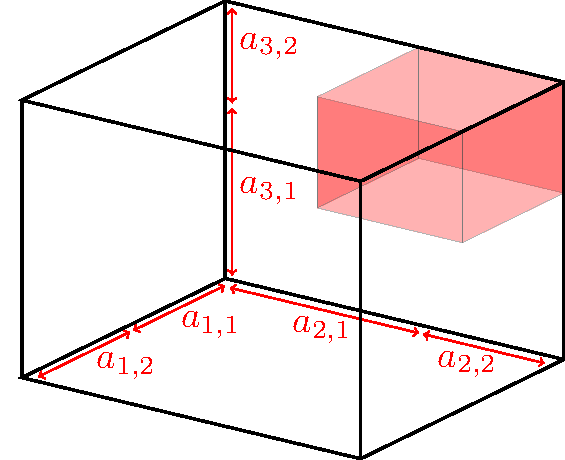
\includegraphics[width=0.4\textwidth]{figures/2/recursion.pdf}
\caption{A recursively constructed $[b_1] \times [b_2] \times [b_3]$ grid, for $n = 2$, $d = 3$.}
\label{fig:recursion}
\end{figure} 

\begin{lem}
\label{lem:recursion}
For $n,d \geq 1$, let $A = (a_{i,j})$ be a $d \times n$ matrix of positive integers, and let $b_i = \sum_{j=1}^n a_{i,j}$, for $1 \geq j \geq d$. Let $S$ be a lethal set under the modified process on $[n]^d$, and for each vertex $\vec{x} = (x_1, \dots, x_v) \in S$, let $T_{\vec{x}}$ be a lethal set on $\prod_{i=1}^d [a_{i,x_i}]$ under $d$-neighbor percolation. Then
$$m(b_1, \dots, b_d, d) \leq \sum_{\vec{x} \in S} |T_{\vec{x}}|.$$
\end{lem}

\begin{proof}
We imagine sub-dividing the $\prod_{i=1}^d [b_{i}]$ brick into smaller blocks by partitioning each of the $d$ axes into segments $a_{i,1}, a_{i,2}, \dots, a_{i,n}$, $1 \leq i \leq d$. Each block is given by a unique product of these segments, and represented by a vector $\vec{x} = (x_1, \dots, x_d) \in [n]^d$. Formally, for each such $\vec{x}$, let $G_{\vec{x}}$ be the block with vertex set
$$\prod_{i=1}^d \{1+ \sum_{j=1}^{x_i -1}a_{i,j}, \dots, \sum_{j=1}^{x_i}a_{i,j} \},$$
and edges between vertices that differ by one in exactly one coordinate. Figure \ref{fig:recursion} illustrates the block $G_{\vec{x}}$ for $\vec{x} = (1,2,2) \in [2]^3$. Observe that $G_{\vec{x}}$ is isomorphic to $\prod_{i=1}^d [a_{i,x_i}]$.

For each $\vec{x} \in S$, let $A_{\vec{x}}$ be the vertices of $G_{\vec{x}}$ corresponding to the vertices of $T_{\vec{x}}$ under isomorphism from $\prod_{i=1}^d [a_{i,x_i}]$ to $G_{\vec{x}}$, and let $A_0 = \cup A_{\vec{x}}$. Observe that $|A_0| = \sum_{\vec{x} \in S} |T_{\vec{x}}|$. We show that $A_0$ is lethal on $\prod_{i=1}^d [b_{i}]$.

By the definition of $T_{\vec{x}}$, for each $\vec{x} \in S$, $A_{\vec{x}}$ is lethal on $G_{\vec{x}}$. Imagine running the $d$-neighbor process until all blocks $G_{\vec{x}}$ are fully infected. We claim that this is sufficient to infect all remaining vertices of $\prod_{i=1}^d [b_{i}]$. Consider the remaining blocks $G_{\vec{x}}$, for $\vec{x} \in [n]^d \setminus S$. Since $S$ is lethal under the modified process, each $G_{\vec{x}}$ is adjacent to fully infected blocks in all $d$ directions. In particular, if we consider expanding out the faces of $G_{\vec{x}}$ towards these infected blocks, the resulting cube has $d$ fully infected faces that share a common corner. It is clear that this structure will infect all the vertices of $G_{\vec{x}}$. Repeating this process on each uninfected region of $\prod_{i=1}^d [b_{i}]$ (as they are exposed under the modified process) ultimately results in all vertices becoming infected. This completes the proof. 
\end{proof}

% Corollary that shows the recursion produces tight bounds on the size of lethal sets, IF all of the constituent blocks are divisibility cases
We note that although the lemma above is true in full generality, we are only concerned with the particular case where $n=2$ and $d=3$. The following corollary proves that the bound in Lemma \ref{lem:recursion} is tight for $n=2$ and $d=3$, if lethal sets on at least three of the constituent blocks are perfect. 

\begin{cor}
\label{cor:recursion}
Let $A=(a_{i,j})$ be a $3 \times 2$ matrix of positive integers, and let $b_i = a_{i,1} + a_{i,2}$ for all $1 \leq i \leq 3$. Then $m(b_1, b_2, b_3, 3)$ is at most
$$m(a_{1,1}, a_{2,1}, a_{3,1}, 3) +  m(a_{1,2}, a_{2,2}, a_{3,1}, 3) + m(a_{1,2}, a_{2,1}, a_{3,2}, 3) + m(a_{1,1}, a_{2,2}, a_{3,2}, 3).$$
Furthermore, this bound is tight if at least 3 of the constituent grids are perfect. 
\end{cor}

\begin{proof}
The upper bound on $m(b_1, b_2, b_3, 3)$ is a direct consequence of Lemma \ref{lem:recursion}, since $(1,1,1), (2,2,1), (2,1,2), (1,2,2)$ is lethal under the modified process on $[2]^3$. 

If all grids are perfect, then:  
\begin{align*}
&m(a_{1,1}, a_{2,1}, a_{3,1}, 3) +  m(a_{1,2}, a_{2,2}, a_{3,1}, 3) + m(a_{1,2}, a_{2,1}, a_{3,2}, 3) + m(a_{1,1}, a_{2,2}, a_{3,2}, 3) \\[10pt]
&= \frac{a_{1,1}a_{2,1} + a_{2,1}a_{3,1} + a_{3,1}a_{1,1}}{3} + \frac{a_{1,2}a_{2,2} + a_{2,2}a_{3,1} + a_{3,1}a_{1,2}}{3} \\
&\qquad\qquad\qquad\qquad\qquad\qquad\quad + \frac{a_{1,2}a_{2,1} + a_{2,1}a_{3,2} + a_{3,2}a_{2,1}}{3} + \frac{a_{1,1}a_{2,2} + a_{2,2}a_{3,2} + a_{3,2}a_{1,1}}{3} \\[10pt]
&= \frac{(a_{1,1} + a_{1,2})(a_{2,1} + a_{2,2}) + (a_{2,1} + a_{2,2})(a_{3,1} + a_{3,2}) + (a_{3,1} + a_{3,2})(a_{1,1} + a_{1,2})}{3} \\[10pt]
&= \frac{b_1b_2+b_2b_3+b_3b_1}{3}.
\end{align*}
Similarly, suppose, without loss of generality, that $(a_{1,1}, a_{2,1}, a_{3,1})$ is optimal and the remaining grids are perfect. Then:
\begin{align*}
&m(a_{1,1}, a_{2,1}, a_{3,1}, 3) +  m(a_{1,2}, a_{2,2}, a_{3,1}, 3) + m(a_{1,2}, a_{2,1}, a_{3,2}, 3) + m(a_{1,1}, a_{2,2}, a_{3,2}, 3) \\[10pt]
&= \ceil*{\frac{a_{1,1}a_{2,1} + a_{2,1}a_{3,1} + a_{3,1}a_{1,1}}{3}} + \frac{a_{1,2}a_{2,2} + a_{2,2}a_{3,1} + a_{3,1}a_{1,2}}{3} \\
&\qquad\qquad\qquad\qquad\qquad\qquad\quad + \frac{a_{1,2}a_{2,1} + a_{2,1}a_{3,2} + a_{3,2}a_{2,1}}{3} + \frac{a_{1,1}a_{2,2} + a_{2,2}a_{3,2} + a_{3,2}a_{1,1}}{3} \\[10pt]
&= \ceil*{\frac{(a_{1,1} + a_{1,2})(a_{2,1} + a_{2,2}) + (a_{2,1} + a_{2,2})(a_{3,1} + a_{3,2}) + (a_{3,1} + a_{3,2})(a_{1,1} + a_{1,2})}{3}} \\[10pt]
&= \ceil*{\frac{b_1b_2+b_2b_3+b_3b_1}{3}}.
\end{align*}
In both cases, we obtain the lower bound $m(b_1, b_2, b_3, 3)$. This completes the proof. 
\end{proof}

\section{Applying the recursion}

% Handle the divisibility cases, and note that certain augmentations to the recursion allow us to obtain non-divisible optimal grids, if we are cautious with regard to the pieces we use.
Corollary \ref{cor:recursion} provides a proscriptive method for constructing optimal and perfect lethal sets recursively, provided the existence of sufficiently many small building blocks. In the following chapter, we use this technique to obtain perfect lethal sets on all $(b_1,b_2,b_3)$ grids, for $b_1,b_2,b_3 \geq 5$, and optimal lethal sets on all $(b_1,b_2,b_3)$ grids, for $b_1,b_2,b_3 \geq 11$. To facilitate this process, we first present some useful constructions of lethal sets (discussed in greater detail in Chapter [Constructions]), as well as particular applications of Corollary \ref{cor:recursion} that hold for general grids. 

\begin{prop}
\label{prop:3x3xk}
For all $k \geq 1$ such that $k \neq 2$, $(3,3,k)$ is perfect.
\end{prop}

\begin{prop}
For all $k \geq 2$, $(3,6,k)$ is perfect.
\end{prop}

\begin{prop}
For all $k \equiv 3 \pmod 6$ and $l \equiv 1 \pmod 2$, $(3,k,l)$ is perfect.
\end{prop}

Combining the above propositions with Corollary \ref{cor:recursion}, we are able to obtain the following lemmas.

\begin{lem}
Suppose $(b_1, b_2, b_3)$ is optimal. Then $(b_1+3, b_2+3, b_3+3)$ is optimal. 
\end{lem}

\begin{proof}
By Proposition \ref{prop:3x3xk}, each of $(b_1,3,3), (3,b_2,3),(3,3,b_3)$ is perfect. Therefore, by Corollary \ref{cor:recursion}, 
$$m(b_1+3, b_2+3, b_3+3, 3) = m(b_1,b_2,b_3,3) + m(b_1,3,3,3) + m(3,b_2,3,3) + m(3,3,b_3,3),$$
and so $(b_1+3, b_2+3, b_3+3)$ is optimal.
\end{proof}

% Example of the recursion on a small grid and discussion re: the strategies for analyzing percolating sets

\section{Examples and Notation}

% Discuss that the recursion works by assembling any set of compatible n^2 blocks, although it is very rare that it is necessary to use more than 4. 
% Talk about the component pieces necessary to assemble a brick of size (a,b,c).

% Should we talk about the broad behavior of percolating sets?
\section{Regional vs. Temporal Infections}

